
% This LaTeX was auto-generated from MATLAB code.
% To make changes, update the MATLAB code and republish this document.

\documentclass{article}
\usepackage{graphicx}
\usepackage{color}

\sloppy
\definecolor{lightgray}{gray}{0.5}
\setlength{\parindent}{0pt}

\graphicspath{ {Assignment_1_files/} }
\begin{document}

    
    
\subsection*{Contents}

\begin{itemize}
\setlength{\itemsep}{-1ex}
   \item Part 1
   \item Part 2
   \item Part 3
\end{itemize}
\begin{verbatim}
%Assignemnt 1
%Brian Hosler and Sarah Peachey
\end{verbatim}


\subsection*{Part 1}

\begin{verbatim}
%1
%The Gcorrection function
type('Gcorrection.m')

%2
%read in the image
pout=imread('Assignment_1_Files/pout.tif');
figure
%Plot .4 enhanced image and histogram
subplot(2,3,1)
imshow(Gcorrection(pout,.4))
title('\gamma=0.4')
subplot(2,3,4)
imhist(Gcorrection(pout,.4))
%Plot unenhanced image and histogram
subplot(2,3,2)
imshow(Gcorrection(pout,1))
title(sprintf('\\gamma=1\nMSE from original: %d',immse(pout,Gcorrection(pout,1))))
subplot(2,3,5)
imhist(Gcorrection(pout,1))
%Plot 2.1 enhanced image and histogram
subplot(2,3,3)
imshow(Gcorrection(pout,2.1))
title('\gamma=2.1')
subplot(2,3,6)
imhist(Gcorrection(pout,2.1))

%3
%Read in new photo
moonHobos=imread('Assignment_1_Files/MoonPhobos.tif');
figure
%Plot the enhanced image
subplot(1,2,1)
imshow(Gcorrection(moonHobos,.3))
title('\gamma=.3')
subplot(1,2,2)
imshow(histeq(moonHobos,256))
title('HistEQ')

figure
%Plot histograms of the enhanced image
subplot(1,2,1)
imhist(Gcorrection(moonHobos,.3))
title('\gamma=.3')
subplot(1,2,2)
imhist(histeq(moonHobos,256))
title('HistEQ')
\end{verbatim}

        \color{lightgray} \begin{verbatim}
function [ img_out ] = Gcorrection(img_in, gama)
%Does gamma correction using the equation:
%   new=2558(old/255)^gamma
    img_out=uint8(255*(double(img_in)/255).^gama);
end

\end{verbatim} \color{black}
    
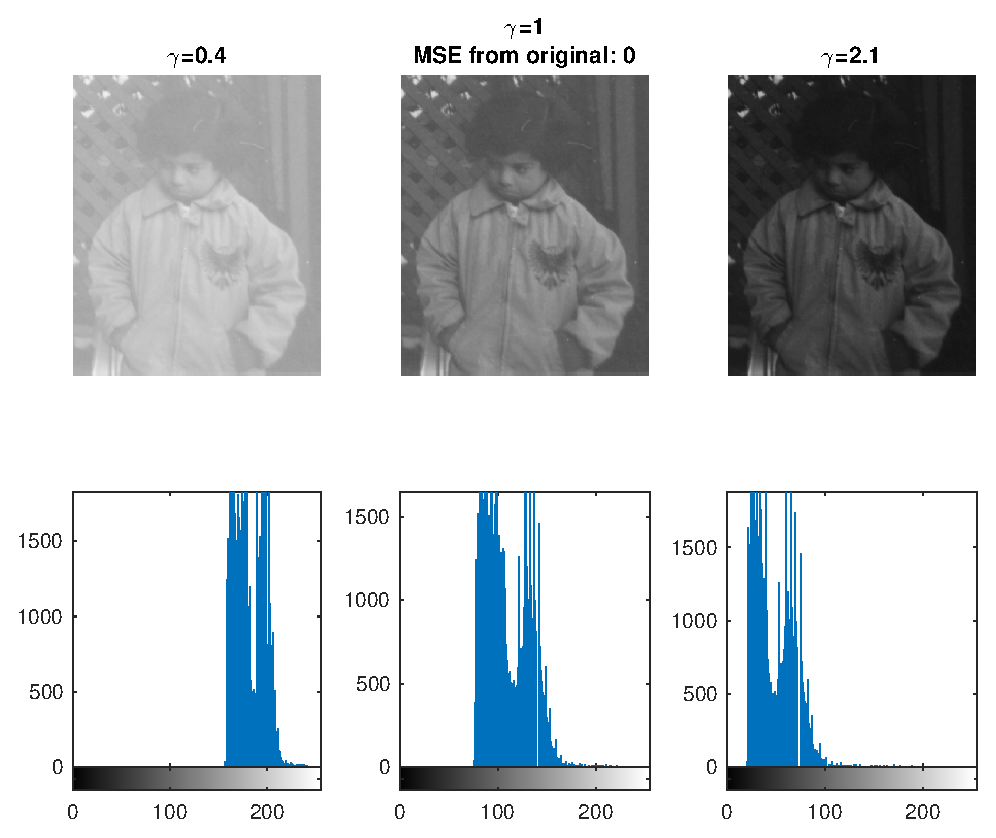
\includegraphics [width=4in]{lab1_01.eps}

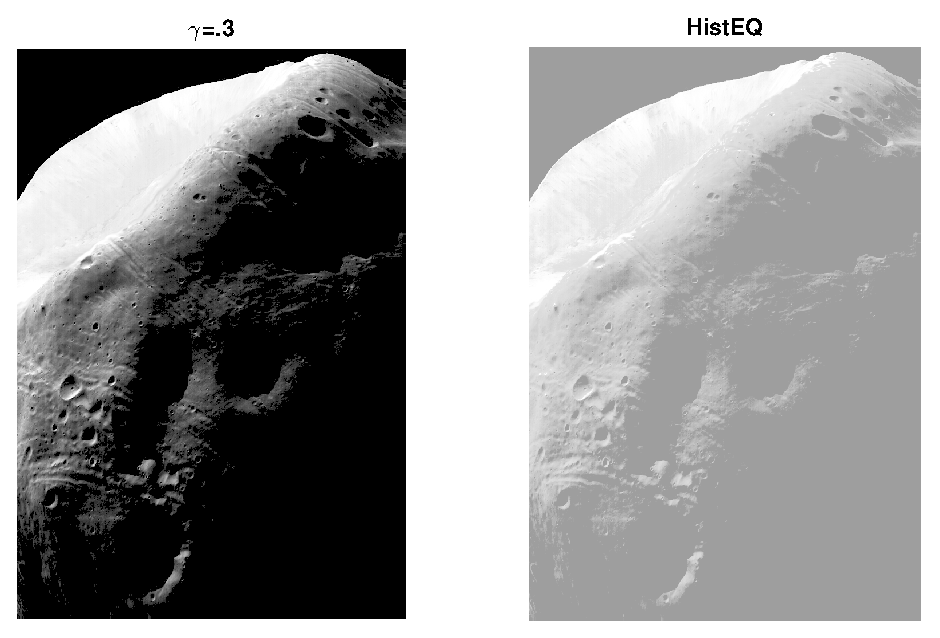
\includegraphics [width=4in]{lab1_02.eps}

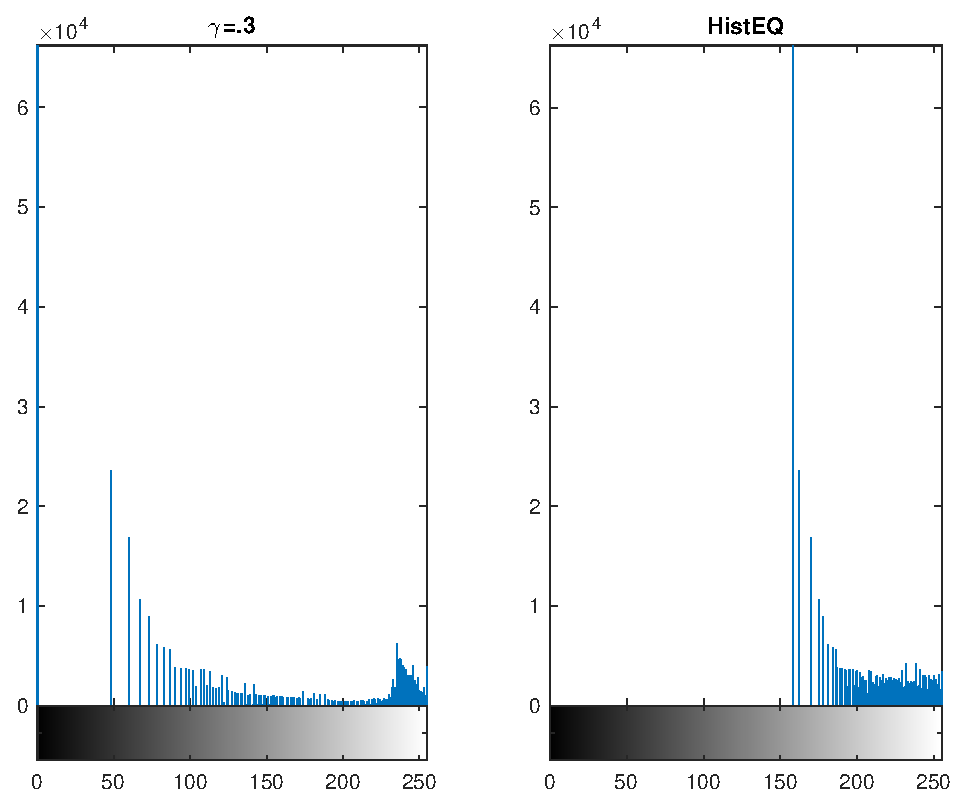
\includegraphics [width=4in]{lab1_03.eps}


\subsection*{Part 2}

\begin{verbatim}
%1
%Our High-Boot filter function
type('HBfilt.m')

%2
%Read in and filter the moon image
moon=imread('Assignment_1_Files/moon.tiff');
figure
imshow(HBfilt(moon,2.4))
title('\alpha=2.4')

%3
%Read in a blurry image and high-boost filter it
oof=imread('Assignment_1_Files/outoffocus.tif');
figure
imshow(HBfilt(oof,4))
title('\alpha=4')
%High frequency noise added with increasing alpha(7)
\end{verbatim}

        \color{lightgray} \begin{verbatim}
function [ img_out ] = HBfilt(img_in, alph)
%High boost filtering using a laplaccian filter
    img_out=img_in+uint8(alph*conv2(double(img_in),[0 -.25 0; -.25 1 -.25; 0 -.25 0],'same'));
end

Warning: Image is too big to fit on screen; displaying at 67% 
\end{verbatim} \color{black}
    
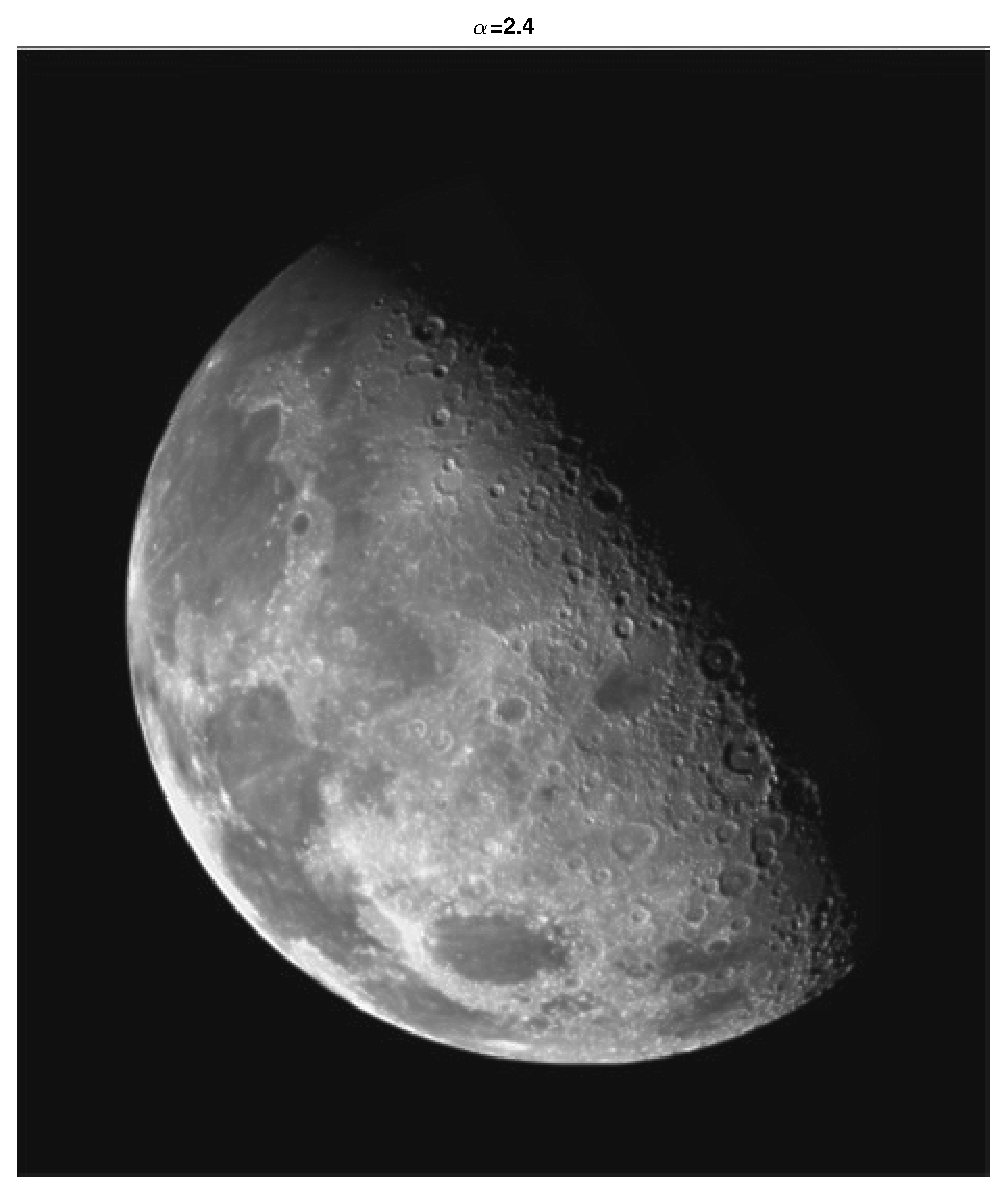
\includegraphics [width=4in]{lab1_04.eps}

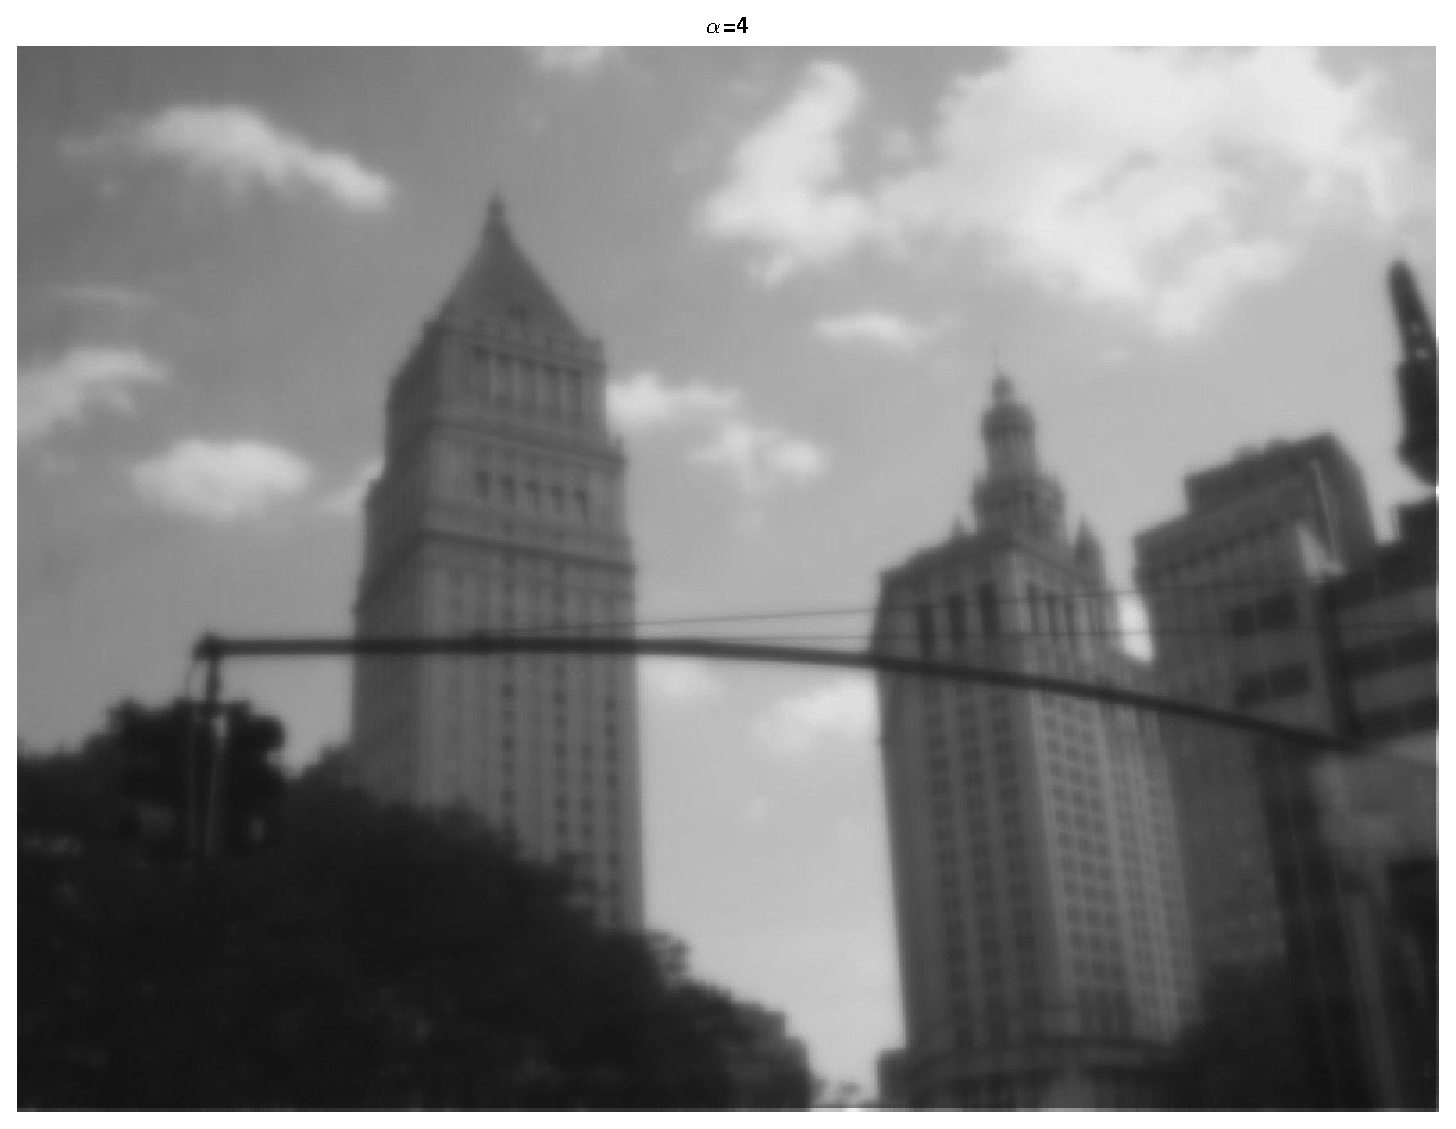
\includegraphics [width=4in]{lab1_05.eps}


\subsection*{Part 3}

\begin{verbatim}
%1
%Read in two noidy images
pep1=imread('Assignment_1_Files/peppersNoise1.tiff');
pep2=imread('Assignment_1_Files/peppersNoise2.tiff');
figure
%Denoise images with a 3x3 median filter
subplot(4,2,1)
imshow(medfilt2(pep1,[3,3]))
title(sprintf('peppersNoise1\nMedian 3x3'))
subplot(4,2,2)
imshow(medfilt2(pep2,[3,3]))
title(sprintf('peppersNoise2\nMedian 3x3'))
%Denoise images with a 5x5 median filter
subplot(4,2,3)
imshow(medfilt2(pep1,[5,5]))
title('Median 5x5')
subplot(4,2,4)
imshow(medfilt2(pep2,[5,5]))
title('Median 5x5')
%Denoise images with a 3x3 averaging filter
subplot(4,2,5)
imshow(uint8(filter2(ones(3,3)/9,pep1)))
title('Averaging 3x3')
subplot(4,2,6)
imshow(uint8(filter2(ones(3,3)/9,pep2)))
title('Averaging 3x3')
%Denoise images with a 5x5 averaging filter
subplot(4,2,7)
imshow(uint8(filter2(ones(5,5)/25,pep1)))
title('Averaging 5x5')
subplot(4,2,8)
imshow(uint8(filter2(ones(5,5)/25,pep2)))
title('Averaging 5x5')

%2
%Save the average and median filtered images
pep1avg=uint8(filter2(ones(3,3)/9,pep1));
pep1med=medfilt2(pep1,[3,3]);
figure
th=60000;
subplot(1,2,1)
sx=filter2([-1,0,1;-2,0,2;-1,0,1],pep1avg).^2;%Xgradient
sy=filter2([-1,0,1;-2,0,2;-1,0,1].',pep1avg).^2;%Ygradient
imshow((sx+sy)>th)%Magnitude squared
subplot(1,2,2)
sx=filter2([-1,0,1;-2,0,2;-1,0,1],pep1med).^2;%Xgradient
sy=filter2([-1,0,1;-2,0,2;-1,0,1].',pep1med).^2;%Ygradient
imshow((sx+sy)>th)%Magnitude squared
\end{verbatim}

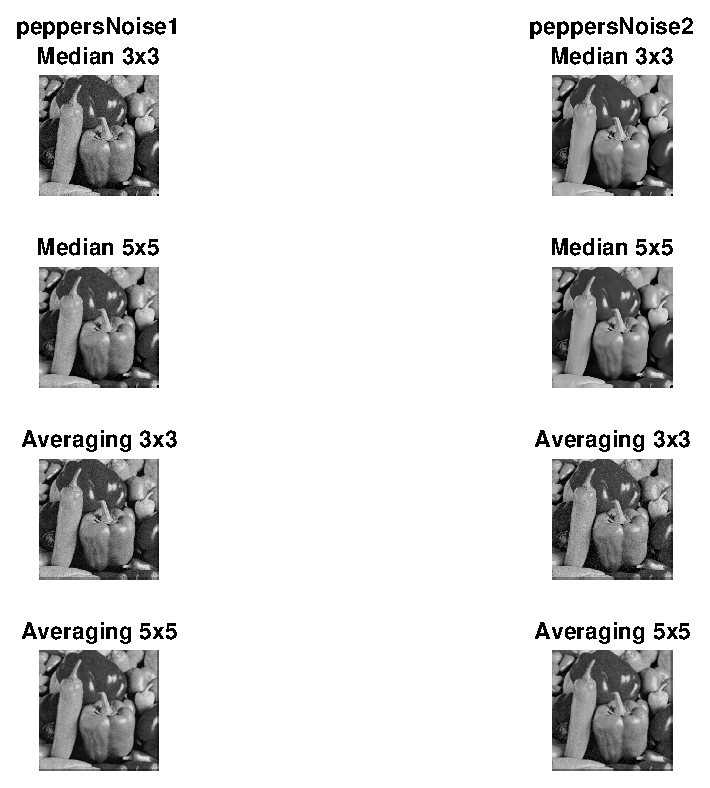
\includegraphics [width=4in]{lab1_06.eps}

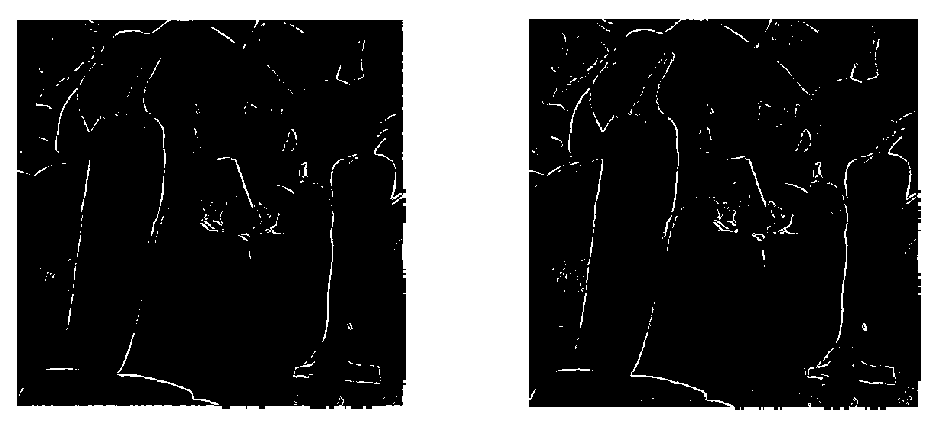
\includegraphics [width=4in]{lab1_07.eps}



\end{document}
    
